\chapter{Planificación y presupuesto}
\section{Metodología}
Durante el transcurso de los estudios del grado, sobre todo en los últimos cursos del mismo, se ha aprendido y profundizado sobre metodologías ágiles, los principios en los que se basan y las herramientas creadas a partir de las mismas. Gracias a lo anterior, y en base a los principios del proyecto en el que se está trabajando, se ha determinado la metodología a seguir durante el desarrollo del mismo.

Como marco de trabajo de desarrollo del proyecto se ha elegido una adaptación propia de Scrum. Aunque Scrum es un marco de trabajo genérico, contiene algunos principios que no son aplicables a la idiosincrasia este proyecto, por ejemplo, los relacionados con la colaboración, asunción de diferentes roles y trabajo en equipo. Esto es debido a que este proyecto se realiza de forma única por el estudiante, con supervisión del tutor, por supuesto, pero sin colaboración activa de otras partes. 

En este marco de trabajo auto-adaptado se han definido los siguientes principios:
\begin{itemize}
    \item 
\end{itemize}
También se han aplicado principios de diseño tales como KISS (Keep It Simple, Stupid!)
Evidentemente, hay 

\section{Herramientas utilizadas}

Java 17 LTS
Jade library
IntelliJ IDE

Latex
Overleaf

Google Drive (Suite)
Drawio
Excel

Google Scholar
Github

StackOverflow

Notion

Telegram

\section{Planificación temporal}

\section{Presupuesto}
La elaboración de un buen presupuesto es una de las partes más importantes en la gestión de proyectos. En multitud de ocasiones, sobre todo si los proyectos son muy grandes, no se tiene un único presupuesto por proyecto, sino que se presupuesta de formas muy variadas, dependiendo, por ejemplo, de la fase en la que se encuentre el proyecto. No es lo mismo que se le quiera proporcionar al cliente un presupuesto inicial, antes de comenzar el proyecto, a que el proyecto se encuentre en una fase avanzada y el cliente solicite nuevas funcionalidades.

Para el proyecto MURAT se ha elaborado un único presupuesto, el cual es suficiente para describir todos los gastos del mismo, los cuales ascienden a un total de 7985 \euro. El presupuesto se ha dividido en tres principales bloques:
\begin{itemize}
    \item \textbf{Personal contratado}: En esta sección se incluyen los gastos conocidos como costes directos, relativos al salario de los empleados. Dentro de esta sección, se pueden diferenciar tres partes principales:
    \begin{itemize}
        \item \textit{Salario bruto}: Es la cantidad total a partir de la cual el trabajador obtiene su sueldo neto previas deducciones por tributación de IRPF y cotización de la Seguridad Social. Se ha estipulado un salario bruto de alrededor de 32.000 \euro \space anuales\footnote{Basado en el sueldo bruto medio de Ingenieros Informáticos en España en el año 2022. Valor obtenido de \href{https://www.glassdoor.es/Sueldos/ingeniero-inform\%C3\%A1tico-sueldo-SRCH_KO0,21.htm}{Glassdoor} a fecha 6 de junio de 2022.}.
        \item \textit{Cuota patronal}: Es la cantidad que la empresa debe pagar por el trabajador. Se compone de los diferentes conceptos: contigencias comunes, 23,60\%; desempleo, 5,50\%; formación profesional, 0,60\%; y FOGASA, 0,20\% \footnote{Basado en el importe mensual que tiene que pagar una compañía en concepto de cuota a la Seguridad Social por tener asalariados contratados. Valores obtenidos de \href{https://www.sdelsol.com/glosario/cuota-patronal/}{Software del Sol} a fecha 6 de junio de 2022.}. Se ha estimado, en total, al 30\% del salario bruto del trabajador.
        \item \textit{Dietas}: Es un extra que en determinadas circunstancias la compañía debe pagar al trabajador. Las dietas son comunes en empresas del sector tecnológico y pueden ser necesarias en cualquier momento. En este caso, no existe ningún gasto relativo a esta parte.
    \end{itemize}
    Este concepto tiene un coste de 6825 \euro \space para el proyecto MURAT.
    \item \textbf{Costes indirectos}: En esta sección se incluyen los gastos generados por el propio ejercicio de la actividad. Es necesario un ordenador portátil, además de un conexión de internet y acceso a la red eléctrica. No  ha sido el caso del proyecto MURAT, aunque en el futuro podría suceder, incurrir en gastos de oficina (o del espacio de trabajo) y de administración, los cuales son prácticamente inherentes a cualquier actividad económica. Este concepto tiene un coste de 1160 \euro \space para el proyecto MURAT.
    \item \textbf{Herramientas y tecnologías}: En esta sección se incluye todo lo relativo a licencias, programas, servicios, etc., necesarios para el proyecto. Esta sección es muy importante en los proyectos de software porque, si bien es cierto que existen muchas herramientas y tecnologías open source gratuitas, existen muchas herramientas y tecnologías propietarias o, incluso, servicios relativos a infraestructura en la nube cuyos costes tienen un impacto considerable en los presupuestos de los proyectos. Este concepto tiene un coste de 0 \euro \space para el proyecto MURAT.
\end{itemize}

\begin{figure}[H]
    \centering
    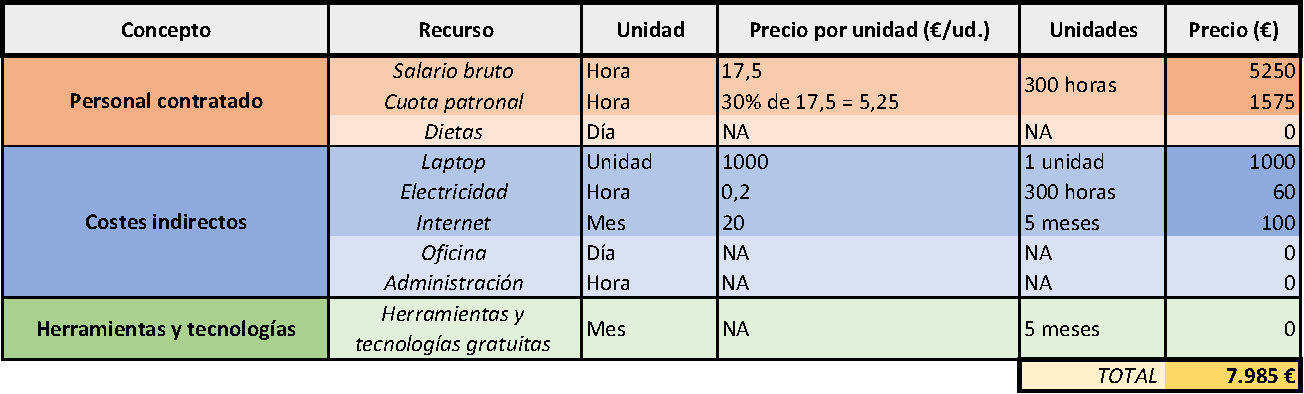
\includegraphics[width=1\linewidth]{text/image/Presupuesto.pdf}
    \caption{Presupuesto del proyecto}
    \label{fig:presupuesto}
\end{figure}